%%%%%%%%%%%%%%%%%%%%%%%%%%%%%%%%%%%%%%%%%%%%%%%%%%%%%%%%%%%%%%%%%%
%%%%%%%% CPSC 66 FALL 2021  REPORT %%%%%%%%%%%%%%%%%%%%%%%%%%
%%%%%%%% This template is modified from ICML 2014 %%%%%%%%%%%%%%%%
%%%%%%%%%%%%%%%%%%%%%%%%%%%%%%%%%%%%%%%%%%%%%%%%%%%%%%%%%%%%%%%%%%

\documentclass{article}

%include any external packages here.  This is similar to loading a
%library in python or C++

% use Times
\usepackage{times}
% For figures
\usepackage{graphicx}
\usepackage{subfigure}
\usepackage[utf8]{inputenc}
\usepackage{longtable}

% For citations
\usepackage{natbib}



% For algorithms and pseudocode
\usepackage{algorithm}
\usepackage{algorithmic}

%Adds hyperlinks to your citations automatically
\usepackage{hyperref}

% Packages hyperref and algorithmic misbehave sometimes.  We can fix
% this with the following command.
\newcommand{\theHalgorithm}{\arabic{algorithm}}

\usepackage[accepted]{icml2014}


% If your title is long (below), use this command to also provide
% short version.  This will go on the top of every page
\icmltitlerunning{Personality Prediction Using Myers Briggs Type Indicator}

\begin{document}

\twocolumn[ %use two column if you need a text to span across the whole page
\icmltitle{ Personality Prediction Using Myers Briggs Type Indicator }

\icmlauthor{Amy Cho}{ycho3@swarthmore.edu}
\icmlauthor{Jisu Han}{jhan3@swarthmore.edu}
\icmlauthor{Jay Jones}{jjones5@swarthmore.edu}
\icmlauthor{Erica Stutz}{estutz1@swarthmore.edu}

\vskip 0.3in
]

\begin{abstract}

This paper presents a machine learning problem aimed at predicting MBTI personality types using a pre-existing dataset from Kaggle that includes users’ social media posts and respective MBTI types. Multiple supervised learning algorithms, including K-Nearest Neighbor, Decision Tree, Support Vector Machine, Logistic Regression, Random Forest, and Naive Bayes, were utilized in the project. The project also included data pre-processing such as addressing class imbalance utilizing SMOTE, data cleaning, and vectorization. The results indicate that the SVM algorithm performed the best among the classifiers tested. This project has important implications for understanding the relationship between social media language and personality, and demonstrates the potential of machine learning in predicting personality traits from online behavior.

\end{abstract}

\section{Introduction}
\label{introduction}

Founded upon Swiss psychiatrist Carl Jung’s personality theory, The Myers-Briggs Type Indicator (MBTI) is a pseudo-scientific instrument used to classify personality types based on how a person processes the world and forms decisions \citep{mcleod23}. Employed by both casual Internet users and large corporations in their recruitment process, the purpose of this assessment is to enhance individuals’ understanding and awareness of themselves and those around them, in hopes of reducing miscommunication and improving decision-making \citep{myers-briggs}. Specifically, determined by self-selected answers to 93 multiple choice questions, the assessment utilizes four separate indices to form 16 unique MBTI or personality types: extroversion/introversion (E-I), sensation/intuition (S-N), thinking/feeling (T-F), and judgment/perception (J-P).

Although the existing MBTI assessment uses self-reported answers to a list of questions, we hypothesized that a person’s personality type may become apparent through their writing style, specifically on social media posts where users have the freedom to document what they feel and are not restricted by a grading system. Individuals also interact with a large number of diverse users on a daily basis. Thus, our goal is to evaluate whether there exists a relationship between a person’s writing style or language on social media and their MBTI type using natural language processing and a variety of machine learning algorithms. By analyzing the accuracies of each classifier, we hope to determine which model is best fit for this specific problem.

Overall, the objective of this project is to train multiple models to evaluate whether MBTIs have a correlation with language styles and behavior online. Additionally, we aim to determine whether any patterns can be detected in specific types and their style of writing by exploring the validity of the classifiers in predicting the personality types. 


\section{Methodology}
\label{methodology}


\begin{figure}[ht]
\vskip 0.2in
\begin{center}
\centerline{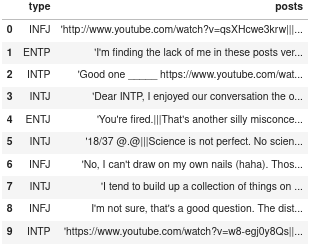
\includegraphics[width=\columnwidth]{image1}}
\caption{First 10 rows of Kaggle dataset.}
\label{data-makeup}
\end{center}
\vskip -0.2in
\end{figure}

For our training dataset, we utilized the existing “(MBTI) Myers-Briggs Personality Type Dataset” from Kaggle. This dataset contains 8674 rows with each row representing an individual user. Each row contains text from 50 social media posts of a given user, each separated by “$||$” , as well as their MBTI type (Figure~\ref{data-makeup}). This data was collected through the PersonalityCafe forum, where users submitted their MBTI types and 50 of their previous social media posts. 

\begin{figure}[ht]
\vskip 0.2in
\begin{center}
\centerline{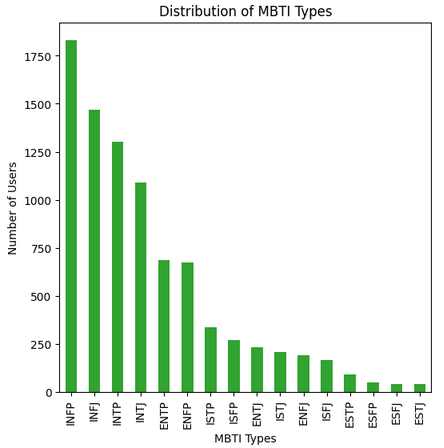
\includegraphics[width=\columnwidth]{image4}}
\caption{Dataset Distribution of MBTI types.}
\label{type-dist}
\end{center}
\vskip -0.2in
\end{figure}

Given that users voluntarily submitted their MBTI types, there exists significant class imbalance within the dataset. As shown in Figure~\ref{type-dist}, 1832 users classify as INFP while only 39 classify as ESTJ. It is also interesting that the majority of sampled users (5697 out of 8674) are classified as introverts. We hypothesize this is because those with introverted tendencies may be more likely to spend increased time on social media, create posts, and submit their MBTI to the PersonalityCafe forum \cite{mitchell17}.

\begin{figure}[ht]
\vskip 0.2in
\begin{center}
\centerline{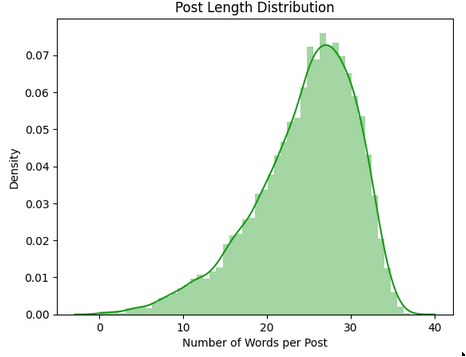
\includegraphics[width=\columnwidth]{image3}}
\caption{Distribution of number of words per individual post.}
\label{post-length-dist}
\end{center}
\vskip -0.2in
\end{figure}

\begin{figure}[ht]
\vskip 0.2in
\begin{center}
\centerline{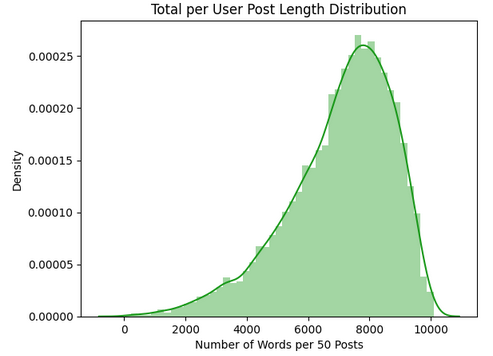
\includegraphics[width=\columnwidth]{image2}}
\caption{Distribution of number of words per user (50 posts).}
\label{50-post-length-dist}
\end{center}
\vskip -0.2in
\end{figure}

Considering that the machine learning classifiers must train on social media posts, we ensured that the posts were of substantial length. Often on social media, users create posts with only one or two words and consequentially, it would be challenging to learn a user’s “writing style” from only a few words. Fortunately, the mean number of words per individual post was 28 words as shown in Figure~\ref{post-length-dist}, and the mean number of words per user (50 posts) is 8000 words Figure~\ref{50-post-length-dist}. Both distributions possess a long left tail indicating that fewer individual posts exist with shorter length.

\subsection{Data Pre-processing: Addressing Class Imbalance}

Given the dataset’s extreme class imbalance and its potential to cause overfitting, we used the Synthetic Minority Oversampling (SMOTE) technique on our training dataset to increase the number of examples within the minority classes. The original imbalanced dataset had a majority class with 1832 samples with 10 other classes containing less than 350 samples each. To correct for the imbalance, we re-sampled by generating synthetic examples ‘near’ existing samples of the minority class \cite{satpathy23}.

This was accomplished by determining nearest neighbor pairs from the under-sampled class and creating synthetic examples at the midpoints between those pairs. More specifically, a numerical value N was chosen to make the different classes in the data have an equal number of examples. From there, an example was randomly selected from each of the minority classes. Subsequently, the K closest examples (we selected K=5) to this random example were found, which were then used to make N new examples by measuring the distance of each K example from the original example and multiplying that by a random number between 0 and 1. We utilized library implementations of the SMOTE algorithm to add synthetic samples to the minority classes (all 15 classes that were not the majority class) which resulted in all 16 classes bearing 1832 samples \cite{satpathy23}.

By reducing the class imbalance, we hypothesized that the classifier accuracy values would be higher, as there is more training data for each MBTI type. Consequently, by skewing the dataset, the accuracy values reflect the real-world dataset less, presenting a tradeoff.


\subsection{Data Pre-processing: Data Cleaning}

We also performed data cleaning to minimize noise by removing links, non English symbols, and any mention of MBTI types in the text data to ensure the machine learning models were training on English words. We were able to do this by using Python’s “re.sub” function to locate all occurrences of links, symbols, and MBTI types and replacing them with an empty string “” or space “ ”. Additionally, we recognized that users may prefer to type in varying cases, so to reduce any issues during training, we converted all words to lowercase using Python’s “.lower()”. Lastly, since the social media posts were collected from the PersonalityCafe forum on which users voluntarily submitted their MBTI types and posts, many users wrote about different MBTI types in their posts. To ensure that the classifiers were not influenced by any mention of MBTI types, we looped through a list of MBTI types and used Python’s “str.replace” function to replace them with a space “ ”.

\subsection{Vectorization}

For data analysis, we chose to utilize Python’s scikit-learn toolkit which possesses several built-in classifier functions. These functions operate primarily with numerical variables rather than categorical ones, which posed an issue for our dataset. As a result, we conducted natural language processing with scikit-learn’s CountVectorizer function. This function transforms text to numerical values by creating a 2-D vector that contains the unique words from the social media posts of the entire dataset as the columns and each of the 8674 user’s posts as the rows. Once this unique word matrix is created, the function loops through each of the users and checks whether or not that user mentioned that specific word in any of their 50 posts. If that specific unique word is present, the respective index’s value in the matrix is set to one, otherwise it is set to zero \cite{using22}. 

\subsection{Employing Classifiers: K-Nearest Neighbor, Decision Tree, Support Vector Machine, Logistic Regression, Random Forest, and Naive Bayes}

Once we completed the natural language processing step, we trained and split the data using scikit-learn’s built-in train\_test\_split function. We chose to conduct a 60/40 train/test split to ensure a large sample set for training and a decently large sample size for testing to reduce the variance in the results of our classifiers. Following, we ran several machine learning classifiers on our data and evaluated their respective accuracies. The supervised learning algorithms we chose to utilize are K-Nearest Neighbor (KNN), Decision Tree, Support Vector Machine (SVM), Logistic Regression, Random Forest (RF), and Naive Bayes (NB). Since we had previously implemented many of these algorithms by-hand, we chose to utilize scikit-learn’s built-in classifier functions for each of the algorithms.

KNN is a machine learning algorithm that predicts the classification of a new data point based on the class of its k-nearest neighbors in the training set. It calculates the Euclidean distance between the new data point and all other points in the training set, and selects the k nearest neighbors based on that distance \cite{kneighbors23, supervisedlearning}.

A Decision Tree is an algorithm that learns a series of if-then-else decisions based on the features of a dataset. The algorithm starts with a root node that represents the entire dataset, and then splits the data into smaller and smaller subsets based on the values of the features. Each split creates a new node in the tree, and this process continues until the algorithm reaches a stopping criteria, such as a minimum number of samples per node or a maximum tree depth. The resulting tree can be used for both classification and regression tasks, and can be visualized to gain insights into how the algorithm is making decisions \cite{decisiontree23, supervisedlearning}.

A Support Vector Machine (SVM) is an algorithm that attempts to find the best possible boundary (or hyperplane) that separates two classes in a dataset. It does this by creating a boundary that maximizes the margin between the classes. The SVM algorithm works by finding a set of support vectors, which are the points closest to the boundary, and then optimizing the boundary to ensure that it separates the classes as well as possible. This method is useful for our problem as it has been shown to be effective in a variety of applications such as text classification \cite{sgdclassifier23, supervisedlearning}.

Logistic regression is an algorithm used for predicting the probability of a binary outcome (i.e., 0 or 1) based on the values of the input features. The algorithm works by fitting a logistic curve to the data, which represents the probability of the binary outcome as a function of the input features. During training, the algorithm adjusts the curve's parameters to minimize the difference between the predicted probabilities and the actual outcomes in the training data. Once trained, the logistic regression model can be used to predict the probability of the binary outcome for new data points, which can then be used to make a binary classification decision (e.g., "yes" or "no") \cite{logisticregression23, supervisedlearning}.

Random Forest is an algorithm that combines multiple decision trees in hopes of generating better predictions. It works by creating a set of decision trees that are each trained on a random subset of the data and a random subset of the input features. During training, the algorithm grows each decision tree by selecting the best feature to split the data at each node. The final prediction is made by combining the predictions of all the trees in the forest. Random Forest is useful for our problem due to its popularity for classification tasks and its ability to handle large datasets \cite{randomforest23, supervisedlearning}.

Naive Bayes is an algorithm that uses Bayes' theorem to make predictions. It works by calculating the probability of each possible outcome given the input features and then selecting the outcome with the highest probability. The algorithm assumes that the input features are independent of each other, which simplifies the calculation of probabilities. During training, the algorithm estimates the probabilities of each feature given each outcome using a set of training data. Naive Bayes is useful for our problem as it is a popular algorithm for classification tasks and is known for its ability to handle high-dimensional data \cite{naivebayes23, supervisedlearning}.

\subsection{Tuning and Training: Model Hyperparameter-tuning and Training Set Optimization}

Although scikit-learn’s classifiers greatly reduced the complexity of our problem, we conducted hyperparameter tuning to ensure each of the classifiers performed with high accuracy. For the K-Nearest Neighbor classifier, we chose to set the number of neighbors to two instead of five, which increased the accuracy to 79.43\%. By tailoring the value of this hyperparameter to the dataset, we were able to produce much better results. For the Decision Tree classifier, an increase in the depth of the tree from 3 to 100 resulted in an increase in accuracy to 57.74\%. The large value for maximum depth of the decision tree is understandable considering the large number of examples in the training set. Furthermore, this change resulted in an increase in compute time, representing a tradeoff between high accuracy and computational complexity.

For the SVM classifier, we utilized stochastic gradient descent for training, which is a method used to update the weights in an effort to minimize the loss function \cite{sgdclassifier23}. Additionally, we adjusted the number of iterations over the training data to 20, which resulted in an increase in accuracy from 76.3\% to 80.35\%. For Logistic Regression, we utilized the multiclass parameter to ensure the classifier performed correctly on our specific problem which includes multiple class labels. For the Random Forest classifier, we adjusted the number of estimators to be 50 from 20 which resulted in an increase in accuracy from 71.93\% to 76.36\%. Lastly, for the Naive Bayes classifier, we switched to a Multinomial Naive Bayes and convert our previously sparsed X array to a denser array using X.toarray(). This resulted in an increase of accuracy to 71.96\%.


\section{Experimental Results}

\begin{table}
\begin{center}
\begin{tabular}{ |p{2cm}| p{1.3cm}| p{1.3cm}| p{1.1cm}| p{1.4cm}| }
\hline
\multicolumn{5}{|c|}{ Supervised Classifier's Accuracy, Precision, and Recall} \\
\hline
Classifier & Accuracy & Precision & Recall & F1 Score \\
\hline
KNN                 & 79.43\% & 74.51\% & 79.41\% & 74.82\% \\
Decision Tree       & 57.74\% & 57.61\% & 58.89\% & 57.90\% \\
SVM                 & 80.35\% & 79.69\% & 80.34\% & 79.34\% \\
Logistic Regression & 79.84\% & 78.79\% & 78.71\% & 78.72\% \\
Random Forest       & 76.36\% & 76.41\% & 76.35\% & 76.11\% \\
Naive Bayes         & 71.96\% & 75.28\% & 71.96\% & 71.88\% \\
\hline
\end{tabular}
\caption{\label{table}Table containing accuracy, precision, and recall values for each of the supervised classifiers.}
\end{center}
\end{table}

As shown in Table~\ref{table}, SVM produced the highest accuracy at 80.35\% and Decision Tree produced the lowest accuracy at 57.74\%. We hypothesized this is because SVM is a far more complex classifier than Decision Trees, and it better able to model this large multiclass dataset. Since accuracy is a summary statistic, we chose to calculate the precision, recall, and F1-score for each of the classifiers. One interesting observation is that the recall values are slightly higher than the precision values for KNN, Decision Tree, and SVM indicating that the classifiers are labeling non-positive cases as positive, resulting in a decrease in precision. Although the difference in precision and recall is minimal, these learners may not appropriately classify a portion of users' MBTI types.


\begin{figure}[ht]
\vskip 0.2in
\begin{center}
\centerline{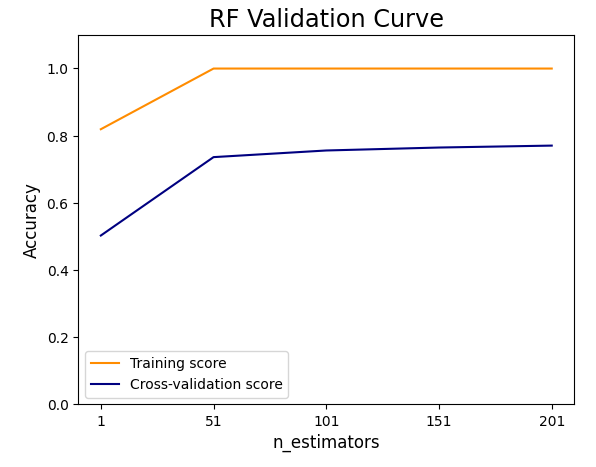
\includegraphics[width=\columnwidth]{image5}}
\caption{Validation Curve for Random Forest}
\label{validation-curve}
\end{center}
\vskip -0.2in
\end{figure}

Additionally, we chose to plot the validation curves of Random Forest, KNN, and SVM to evaluate the effect of our hyperparameter tuning on classifier performance. Based on Figure~\ref{validation-curve}, it is evident that for Random Forest having more estimators correlates to increased accuracy. However, since the cross-validation score is lower than the training score, we can infer that the model shows signs of overfitting.

\begin{figure}[ht]
\vskip 0.2in
\begin{center}
\centerline{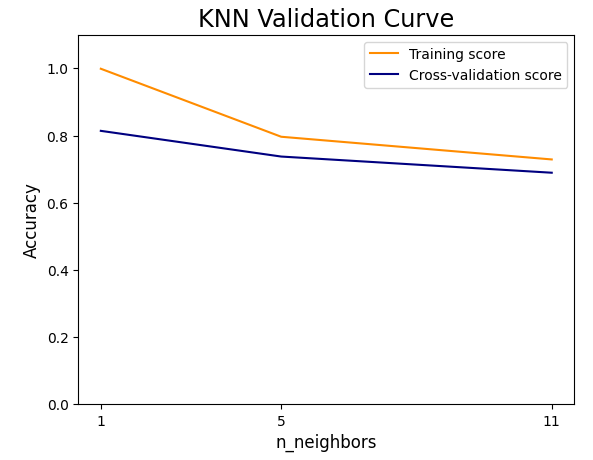
\includegraphics[width=\columnwidth]{image6}}
\caption{Validation Curve for KNN}
\label{knn-curve}
\end{center}
\vskip -0.2in
\end{figure}

Based on Figure~\ref{knn-curve}, having a lower number of neighbors for KNN performs well on the test set. There is not enough discrepancy between the accuracy of the training score and cross validation score results to conclude that the model overfit the training data.

\begin{figure}[ht]
\vskip 0.2in
\begin{center}
\centerline{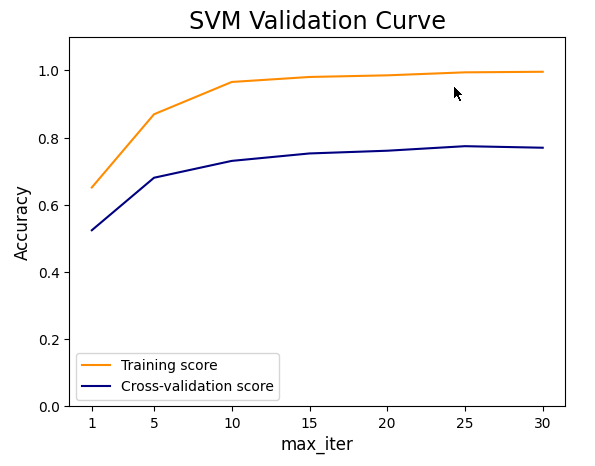
\includegraphics[width=\columnwidth]{image7}}
\caption{Validation Curve for SVM}
\label{svm-curve}
\end{center}
\vskip -0.2in
\end{figure}

Based on Figure~\ref{svm-curve}, increasing the number of iterations for SVMleads to an increase in performance for both the training set and testing set. However, it can be more susceptible to overfitting as shown by the bigger discrepancy between the training and cross validation scores.

From these validation curves and associated precision/recall values, we concluded that the SVM classifier performed best on our dataset while Decision Trees performed the worst. Given that the highest accuracy is approximately 80\%, it would be optimal to raise this value, possibly through additional hyperparameter tuning or creation of a larger training set, before deployment into the real world. 

\section{Social Implications}
\label{social implications}

Our project has a wide array of potential implications in the real world. In recent years, companies have begun to hire people based on MBTI personality types, or at least consider them heavily \cite{nguyen18}. This is done in an effort to promote a healthy work environment filled with coworkers of diverse and compatible personality types, as well as providing employers a level of confidence that potential employees will be a good fit to the company culture \cite{nguyen18}. With the ever-growing prevalence of social media in our daily lives, our project grants firms the opportunity to gain a better understanding of who they are considering hiring during the recruitment process based on their social media presence.

Another potential application is in targeted advertising or recommender systems. Platforms like Meta, Instagram, Twitter, Spotify, Netflix, etc. take advantage of user data in order to better individualize each user’s experience. Whether it be advertising a product or simply recommending a song/movie, awareness and knowledge of a user’s personality type can be valuable information to these platforms. Our project would allow these firms to better cater to users through recommended products or content and in turn, increase profits. This could also be a step in the right direction to developing a solution to the diversity vs. similarity problem that many recommender systems struggle with \cite{solving23}.

Additionally, the MBTI assessment provides individuals with the opportunity to better understand their own communication preferences as well as their cohorts’. By identifying what MBTI type a given user possesses by their writing style on social media posts, users can develop a greater understanding for other’s point of views and how they may process events occuring in the world.

There are, however, a few ethical considerations we must be aware of when developing and employing a program such as this. First, some people may view this as a privacy violation because  personal information and online behavior may be analyzed without the user’s knowledge or consent. This may also lead to discrimination; as discussed earlier, employers have been taking into consideration personality types when hiring. When organizations use the results for decision-making purposes, this can lead to discrimination against certain individuals, which is especially problematic if our algorithm fails to produce the correct result or the data itself is biased. Similarly, a certain level of bias can be exhibited based on the training data used. If our dataset is not representative of the entire population, the model may produce biased results that are skewed.

Finally, given that the current peformance of SVM has approximately 80\% accuracy, users' should be wary to place complete trust in the MBTI type that the classifier outputs based on their social media posts. Mislabeling of MBTI types could lead users to focus on aspects of their personality that do not present as dominant, eliminating the purpose of the MBTI assessment, and could lead to reduced understanding and compassion between users.

\section{Conclusions}
\label{conclusions}

Thus far, we have explored the appropriateness of various supervised learning techniques to predict someone’s MBTI personality type based on social media posts. We found that while Naive Bayes and Random Forests produced fairly decent results, Logistic Regression, KNN, and SVM were most effective with success rates of over 78\% accuracy; the best performing classifier was SVM with 80.35\% accuracy. On the other hand, Decision Tree was far from suitable for this particular type of text classification problem.

Potential improvements to our model may include the use of deep learning techniques such as recurrent neural networks, which perform well on text classification as they are specialized to identify patterns across time-series data. Furthermore, we could extend our project to do the reverse of the process it currently does. Instead of using text as input and outputting an MBTI type, it would take an MBTI type as input and output text. This would bean interesting extension and could be practical in various cases. For instance, a platform could improve customer service and further individualize user experiences by producing responses in a way that matches a user’s personality. This provides a more engaging and personalized experience that seems more conversational and more closely resembles human-like interaction forusers. By understanding a user’s personality, platforms can ensure that they are responding and delivering content in a way that is empathetic and tailored to a user’s needs.


\bibliographystyle{icml2014}
\bibliography{references}

\end{document}


% This document was modified from the file originally made available by
% Pat Langley and Andrea Danyluk for ICML-2K. This version was
% created by Lise Getoor and Tobias Scheffer, it was slightly modified
% from the 2010 version by Thorsten Joachims & Johannes Fuernkranz,
% slightly modified from the 2009 version by Kiri Wagstaff and
% Sam Roweis's 2008 version, which is slightly modified from
% Prasad Tadepalli's 2007 version which is a lightly
% changed version of the previous year's version by Andrew Moore,
% which was in turn edited from those of Kristian Kersting and
% Codrina Lauth. Alex Smola contributed to the algorithmic style files.
